\documentclass[english,compress]{beamer}

\usepackage{amsmath}
\usepackage{amssymb}
\usepackage[english]{babel}
\usepackage{tikz}
\usepackage{mathtools}
\usepackage{graphicx}
\usepackage{subfigure}
\usepackage{beamerthemeMadrid}
\usepackage{default}
\usepackage[square,numbers]{natbib}

\renewcommand{\bibsection}{\subsection*{\bibname}}

%Adding more spacing in itemize
\newlength{\wideitemsep}
\setlength{\wideitemsep}{\itemsep}
\addtolength{\wideitemsep}{5pt}
\let\olditem\item
\renewcommand{\item}{\setlength{\itemsep}{\wideitemsep}\olditem}

% Beamer options
\setbeamertemplate{section page}
{
	\begin{centering}
	\begin{beamercolorbox}[sep=12pt,center]{part title}
	\usebeamerfont{section title}\insertsection\par
	\end{beamercolorbox}
	\end{centering}
}
\beamertemplatenavigationsymbolsempty
\AtBeginSection{\frame{\sectionpage}}
\addtobeamertemplate{navigation symbols}{}{%
    \usebeamerfont{footline}%
    \usebeamercolor[fg]{footline}%
    \hspace{1em}%
    \insertframenumber/\inserttotalframenumber
}
\useoutertheme{split}
\useinnertheme{rectangles}
\usecolortheme{uiuc}
\logo{
\includegraphics[height=0.5cm]{uiuclogo.pdf}}
\expandafter\def\expandafter\insertshorttitle\expandafter{%
    \insertshorttitle\hfill\insertframenumber\,/\,\inserttotalframenumber}

\newcommand{\norm}[1]{\left\lVert #1 \right\rVert}
\newcommand{\abs}[1]{|#1|}
\newcommand{\vect}[1]{\boldsymbol{\mathbf{#1}}}
\newcommand{\ceil}[1]{\left \lceil #1 \right \rceil }
\newcommand{\floor}[1]{\left \lfloor #1 \right \rfloor }
\newcommand{\q}{ {\bf q} }

\title{Parallel Belief Propagation}
\subtitle{Image Super-Resolution}
\date{December 9, 2014}
\author{Nate Bowman, Erin Carrier, Anirudh Jayakumar, Ralf Gunter}

\begin{document}
\nocite{*}

\frame{\titlepage}
\frame{\frametitle{Table of contents}\tableofcontents}
\frame{\frametitle{Overview}
\begin{itemize}
\item Algorithm designed to improve resolution of images
\item Pixel-based images used as input
\item Standard algorithms produce blurry images
\item Large images created from small images
\end{itemize}
}

\frame{\frametitle{Properties and Goals of the Algorithm}
	\begin{itemize}
	\item Uses machine learning
	\item Operates in one pass
	\item Creates plausible high-frequency details
	\item Estimates details unobtainable by simple sharpening
	\end{itemize}
}

\frame{\frametitle{Training}
		\begin{itemize}
		\item Learns fine details corresponding to image regions seen at low
		resolution
		\item Generates low-resolution image: \\
			\framebox{high} $\xrightarrow{blur+subsample}$
			\framebox{small} $\xrightarrow{interpolate}$ \framebox{low}
		\item Creates high-frequency patch: \\
			( \framebox{high} - \framebox{low} ) $\rightarrow$ \framebox{patch}
		\item Stores association: \\
			\begin{tabular}{| c | c |}
				\hline
				low & patch \\
				\hline
			\end{tabular}
		\end{itemize}
}

\frame{\frametitle{Training Optimizations}
	\begin{itemize}
	\item Keeps only highest frequencies of low-resolution images
	\item Locally normalizes contrast to reduce duplicates
	\end{itemize}
}

\frame{\frametitle{Naive Algorithm}
	\begin{itemize}
	\item Interpolates image (e.g., with cubic spline)
	\item Adds high-frequency patches corresponding to best
	match from the training set for each low-resolution patch
	\item Fails due to lack of neighborhood information
	\end{itemize}
}

\frame{\frametitle{Markov Network}
	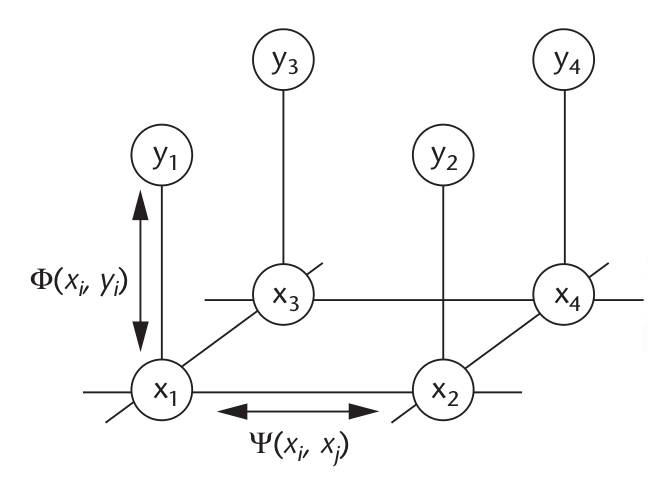
\includegraphics[width=.8\linewidth]{images/markov}
}

\frame{\frametitle{Markov Networks}
	\begin{itemize}
	\item $x_i$: Unknown high-frequency patch. Modeled as a random variable. \\
		$x_i = \left\{\fbox{Patch}, \fbox{Patch}, \hdots, \fbox{Patch}\right\}$
	\item $y_i$: Observed low-resolution patch
	\item $P(x|y) = \frac{1}{Z}\prod_{(ij)}\psi_{ij}(x_i, x_j)\prod_i\phi_i(x_i, y_i)$
	\item $d_{ij}(x_i, x_j)$: sum of squared differences in overlap region
	\item $\psi_{ij}(x_i, x_j) = \exp(-\frac{d_{ij}(x_i, x_j)}{2\sigma^2})$
	\item Similar formula for $\phi_i(x_i, y_i)$
	\end{itemize}
}

\frame{\frametitle{Belief Propagation}
	\begin{itemize}
	\item Fast iterative algorithm
	\item Message: $m_{ij}(x_j)=\sum_{x_i}\psi_{ij}(x_i, x_j)\prod_{k \ne j}m_{ki}(x_i)\phi_i(x_i,y_i)$
	\item Belief: $b_i(x_i)=\prod_km_{ki}(x_i)\phi_i(x_i,y_i)$
	\end{itemize}
}

\frame{\frametitle{Overall Algorithm}
	\begin{itemize}
	\item Interpolate image
	\item Break blurry image into patches
	\item Solve for maximum probability in Markov network
	\item Undo earlier removal of contrast in patches
	\item Add resulting high-frequency patches to blurry image
	\end{itemize}
}

\frame{\frametitle{Example Image}
	\centering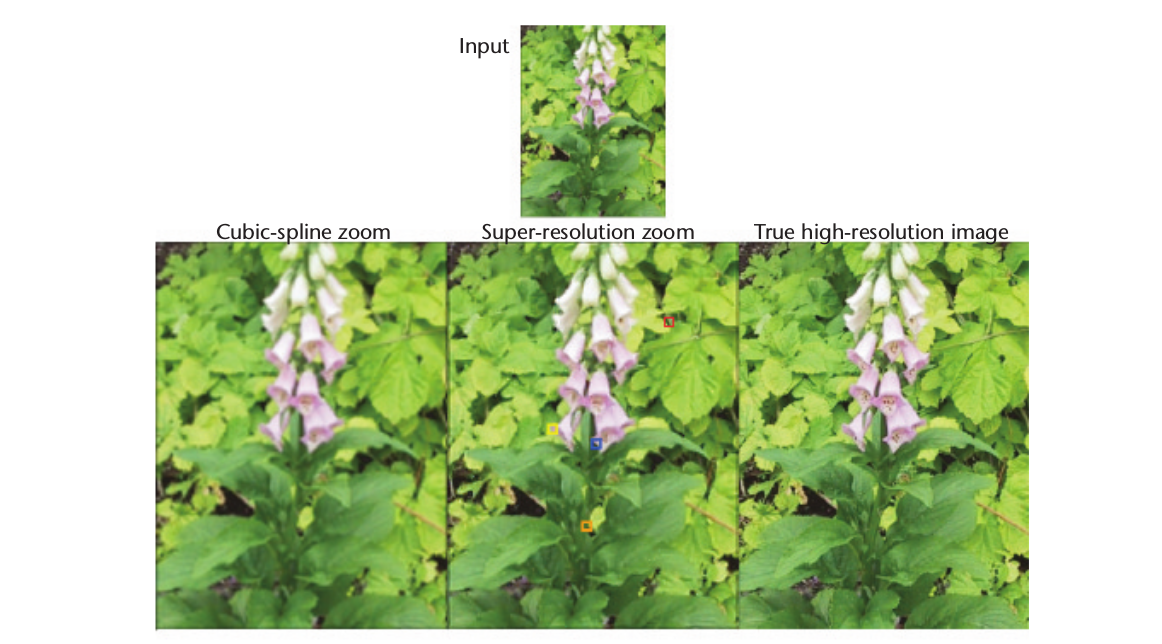
\includegraphics[scale=.25]{images/flower}
}

\frame{\frametitle{Example Image}
	\begin{center}
	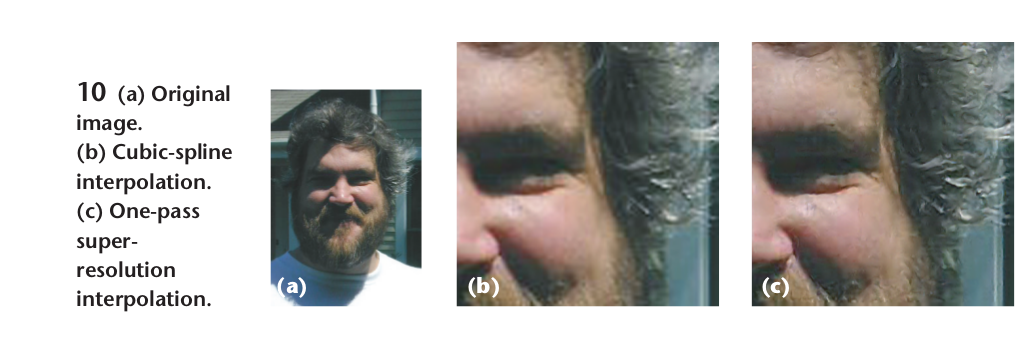
\includegraphics[scale=.3]{images/beard}
	\end{center}
}

\frame{\frametitle{Results}
	\begin{itemize}
	\item Leads to an image that:
		\begin{itemize}
		\item is a good match for each patch
		\item maintains overall look of original image
		\item contains high-resolution features
		\end{itemize}
	\item Can add a weighting factor to favor $\phi$ or $\psi$
	\item Uses a generic training set
	\end{itemize}

}


%\input{}
\section{Introduction}
\section{Image Super-Resolution}
\subsection{Algorithm}
\frame{\frametitle{FrameTitle1}
	\begin{itemize}
	\item Item1
	\item Item2
	\item Item3
	\end{itemize}
}

\frame{\frametitle{FrameTitle2}
	\begin{itemize}
	\item Item1
	\item Item2
	\end{itemize}
}

\section{Our Implementation}
\subsection{Overview}
\frame{\frametitle{Phases}
	\begin{itemize}
	\item Item1 \cite{fp}
	\item Item2
	\end{itemize}
}
\subsection{Preprocessing}
\frame{\frametitle{}
	\begin{itemize}
	\item Item1 \cite{fp}
	\item Item2
	\end{itemize}
}
\subsection{Parallel Belief Propagation}
\frame{\frametitle{Program Flow}
	\begin{itemize}
	\item Item1 \cite{fp}
	\item Item2
	\end{itemize}
}
\subsection{Postprocessing}
\frame{\frametitle{Program Flow}
	\begin{itemize}
	\item Item1 \cite{fp}
	\item Item2
	\end{itemize}
}

\frame{\frametitle{References}
	\bibliographystyle{plainnat}
	\bibliography{bibentries}
}
\end{document}
